\documentclass[10pt,a4paper]{report}
\usepackage[utf8]{inputenc}
\usepackage[german]{babel}
\usepackage[T1]{fontenc}
\usepackage{amsmath}
\usepackage{amsfonts}
\usepackage{amssymb}
\usepackage{graphicx}
\usepackage{listings}
\usepackage{color}
\author{Julian Sobott (76511), David Sugar (76050), Lukas Mendel (76509)}
\title{Bericht Datenbank Praktikum}



\usepackage{geometry}
 \geometry{
 a4paper,
 total={170mm,257mm},
 left=20mm,
 top=20mm,
 }



\lstset{
	language=sql,
	tabsize=4,
	keywordstyle=\color{blue},
	breaklines=true
}	
\begin{document}
\maketitle
\tableofcontents

\newpage
\section{Aufgabe 1}
\subsection{a)}


\begin{figure}[ht!]
	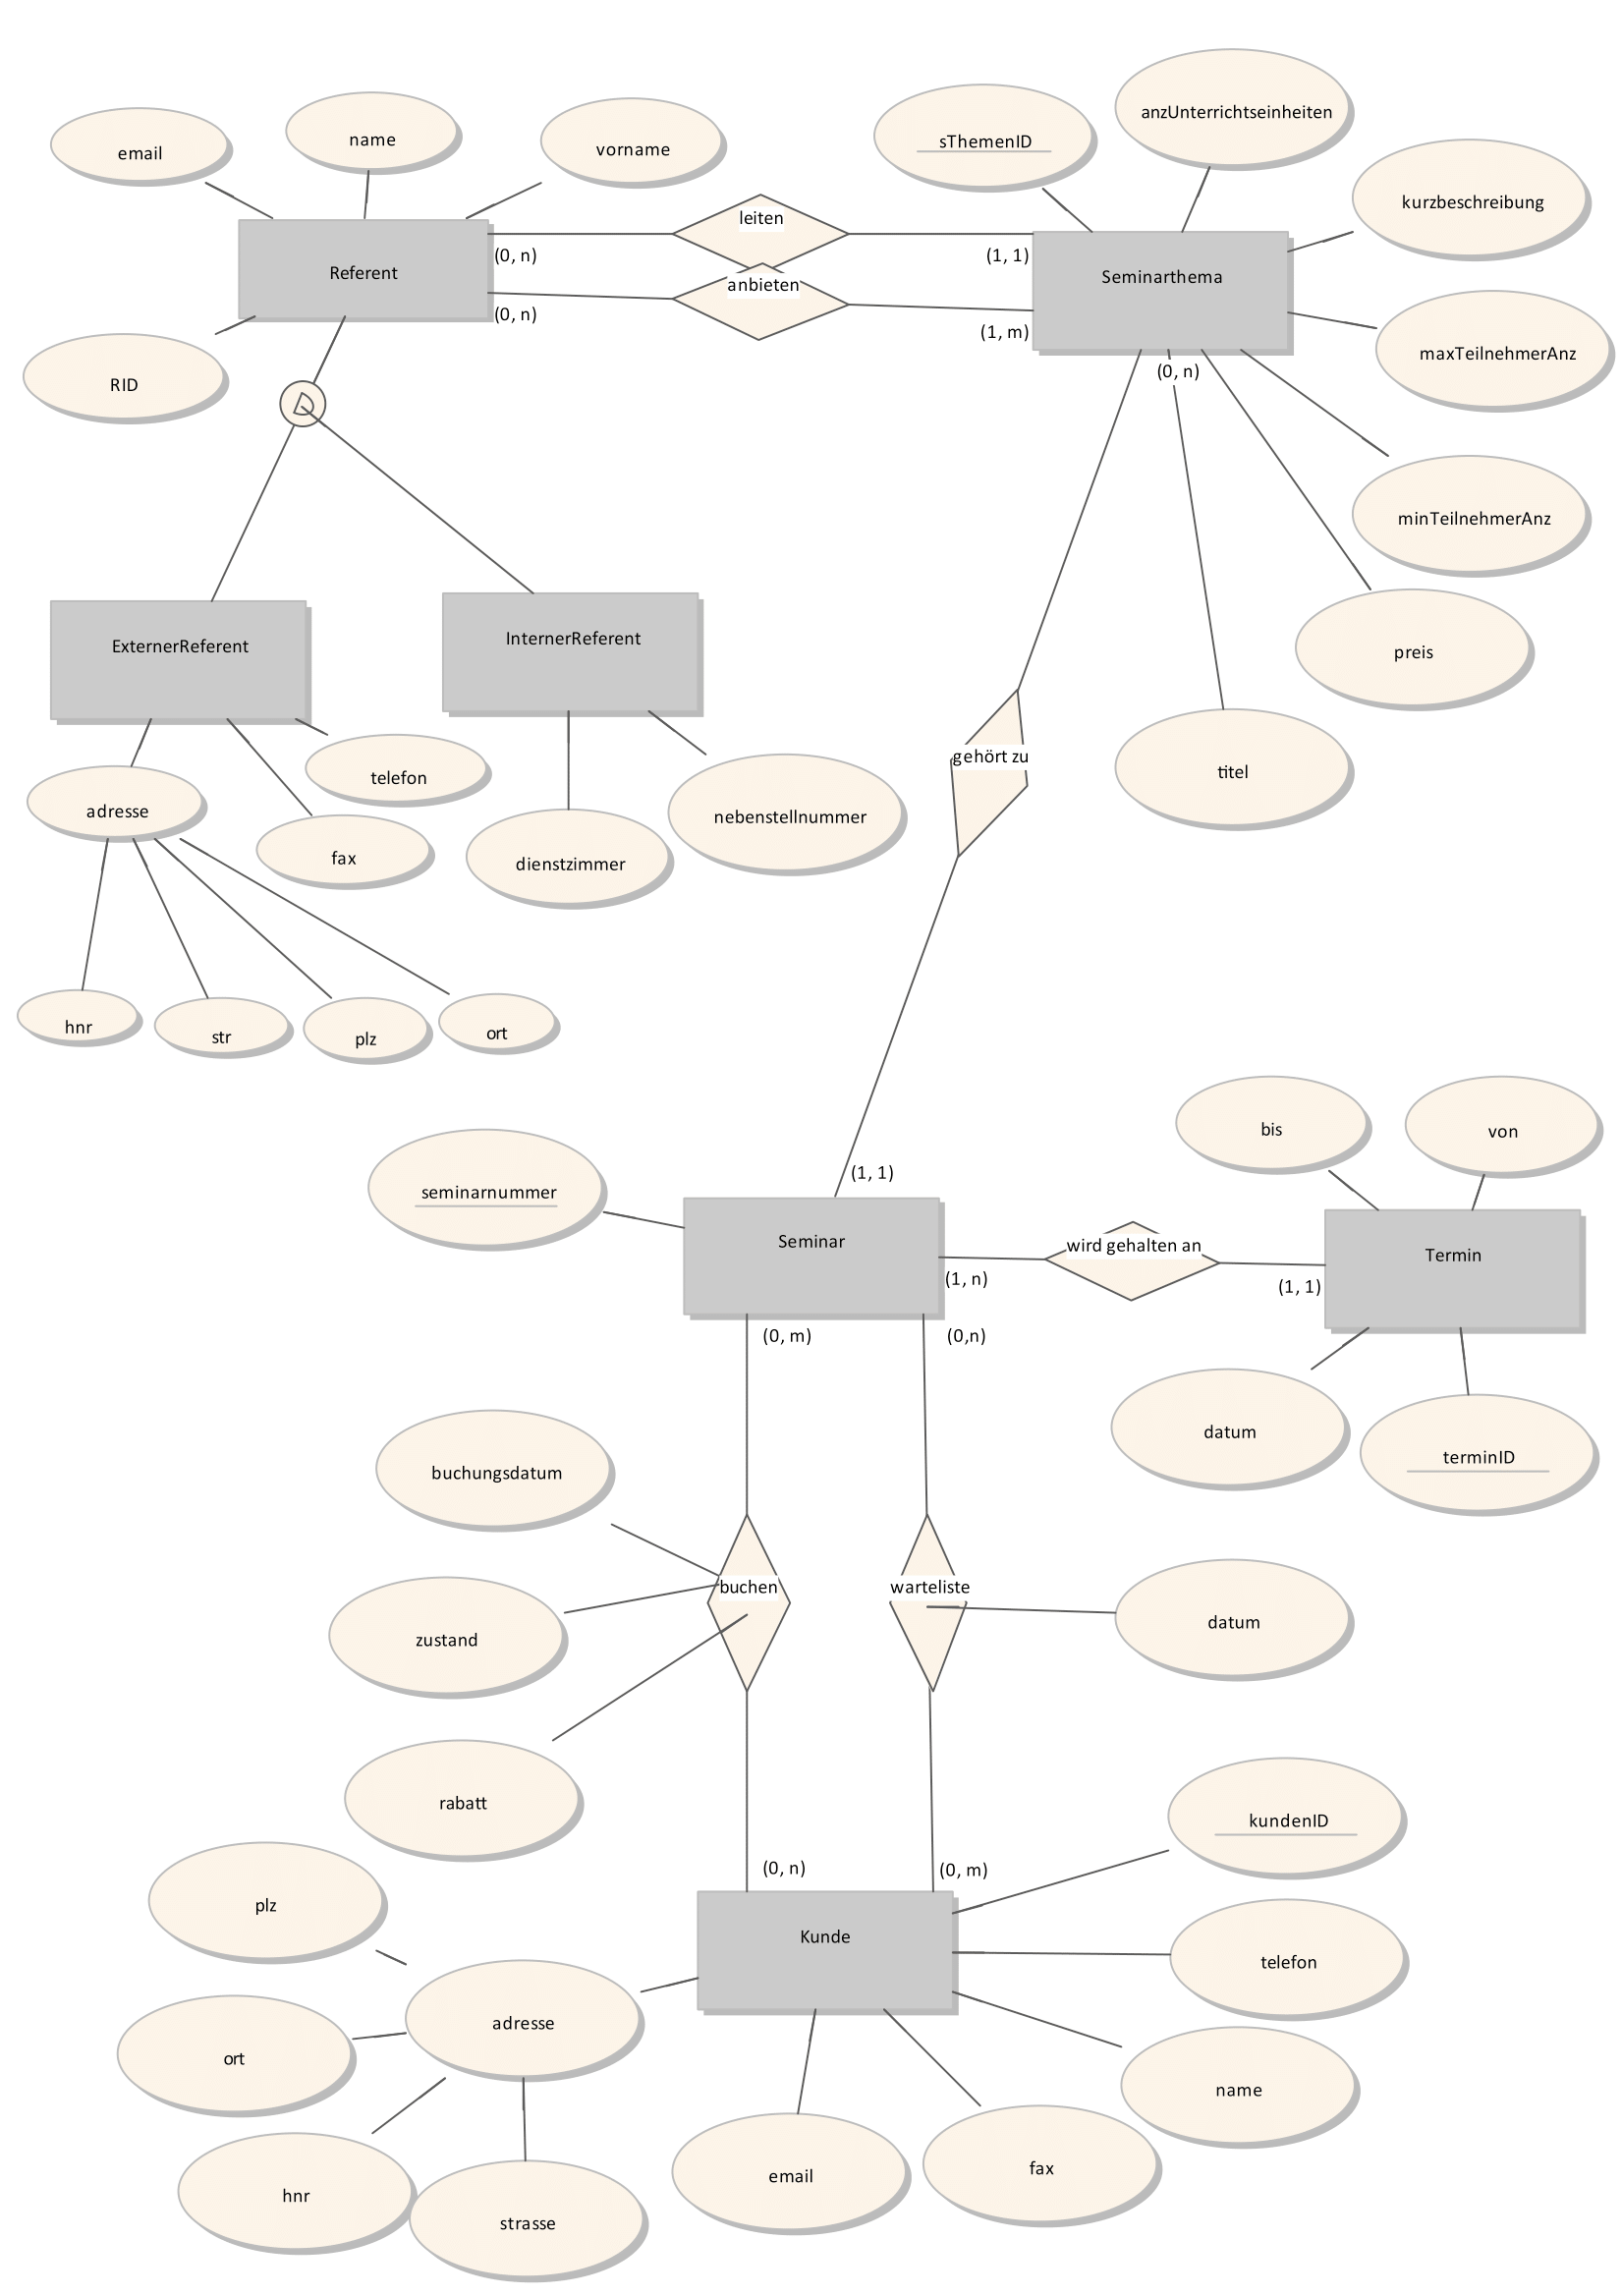
\includegraphics[scale=0.2]{Bilder/ER-Modell.PNG}
	\caption{ER-Modell Seminarverwaltung}
	\label{er:1}
\end{figure}
\newpage
\subsubsection{Entities}
seminar = (\{\underline{SEMINARNUMMER:INTEGER}\})

termin  = (\{\underline{TERMINID:INTEGER}, DATUM:DATE, VON:DATETIME, BIS:DATETIME\})

kunde   = (\{\underline{KUNDENID:INTEGER}, TELEFON:VARCHAR, NAME:VARCHAR, FAX:VARCHAR, EMAIL:VARCHAR, ADRESSE:(PLZ:VARCHR, ORT:VARCHAR, HNR:VARCHAR, STR:VARCHAR)\})

referent = (\{\underline{RID:INTEGER}, email: VARCHAR, name: VARCHAR, vorname: VARCHAR\})

seminarthema = (\underline{STHEMAID:INTEGER}, ANZUNTERICHTSEINHEITEN:INTEGER, KURZBESCHREIBUNG:VARCHAR, MAXTEILNEHMERANZ:INTEGER, MINTEILNEHMERANZ:INTEGER, PREIS:FLOAT, TITEL:VARCHAR\})

externerReferent = (\{\underline{RID:INTEGER},adresse: (plz: VARCHAR, ort: VARCHAR, strasse: VARCHAR, hnr: VARCHAR)\} is\_a referent)

internerReferent = (\{\underline{RID:INTEGER},dienstzimmer: VARCHAR, nebenstellnummer: Integer\} is\_a referent)

\subsubsection{Relations}

leiten = (referent X seminarthema)

anbieten = (referent X seminarthema)

gehört\_zu = (seminarthema X seminar)

buchen = (seminar x kunke, BUCHUNGSDATUM:DATE, ZUSTAND:VARCHAR, RABATT:FLOAT)

warteliste = (kunde x seminar, POSITION:INTEGER)

wird\_gehalten\_an = (seminar x termin)


\subsection{b)}
\subsubsection{Relationen}
referent = (\underline{RID:INTEGER}, email: VARCHAR, name: VARCHAR, vorname: VARCHAR)

ExternerReferent(\underline{RID:INTEGER}, plz: VARCHAR, ort: VARCHAR, strasse: VARCHAR, hnr: VARCHAR)

IntererReferent (\underline{RID:INTEGER}, dienstzimmer: VARCHAR, nebenstellnummer: Integer) 

seminarthema = (\underline{STHEMAID:INTEGER}, ANZUNTERICHTSEINHEITEN:INTEGER, KURZBESCHREIBUNG:VARCHAR, MAXTEILNEHMERANZ:INTEGER, MINTEILNEHMERANZ:INTEGER, PREIS:FLOAT, TITEL:VARCHAR, LEITER:INTEGER)

anbieten = (\underline{REFERENTID:INTEGER, SEMINARTHEMAID:INTEGER})

seminar = (\underline{SEMINARNUMMER:INTEGER}, SEMINARTHEMAID:INTEGER)

termin = (\underline{TERMINID:INTEGER}, VON:DATETIME, BIS:DATETIME, DATUM:DATE, SEMINARID:INTEGER)

kunde   = (\underline{KUNDENID:INTEGER}, TELEFON:VARCHAR, NAME:VARCHAR, FAX:VARCHAR, EMAIL:VARCHAR, PLZ:VARCHR, ORT:VARCHAR, HNR:VARCHAR, STR:VARCHAR)

buchen = (\underline{KUNDENID:INTEGER, SEMINARNR:INTEGER}, BUCHUNGSDATUM:DATE, ZUSTAND:VARCHAR, RABATT:FLOAT)

warteliste = (\underline{KUNDENID:INTEGER, SEMINARNR:INTEGER}, POSTION:INTEGER)

\subsubsection{Referenzen}
$seminarthema\vert_{LEITER} \subseteq refernet\vert_{RID}$

$anbieten\vert_{REFERENTID} \subseteq refernet\vert_{RID}$

$anbieten\vert_{SEMINARTHEMAID} \subseteq seminarthema\vert_{STHEMAID}$

$seminar\vert_{SEMINARTHEMAID} \subseteq seminarthema\vert_{STHEMAID}$

$termin\vert_{SEMINARID} \subseteq seminar\vert_{SEMINARNUMMER}$

$buchen\vert_{KUNDENID} \subseteq kunde\vert_{KUNDENID}$

$buchen\vert_{SEMINARNR} \subseteq seminar\vert_{SEMINARNR}$

$warteliste\vert_{KUNDENID} \subseteq kunde\vert_{KUNDENID}$

$warteliste\vert_{SEMINARNR} \subseteq seminar\vert_{SEMINARNR}$

\subsection{c)}

\lstinputlisting{../create_table_statements.sql}

\section{Aufgabe 2}
\lstinputlisting{../insert_table_statements.sql}

\section{Aufgabe 3}
\lstinputlisting{../SQL_Abfragen.sql}

\section{Aufgabe 4}
\subsection{a)}


\begin{figure}[ht!]
	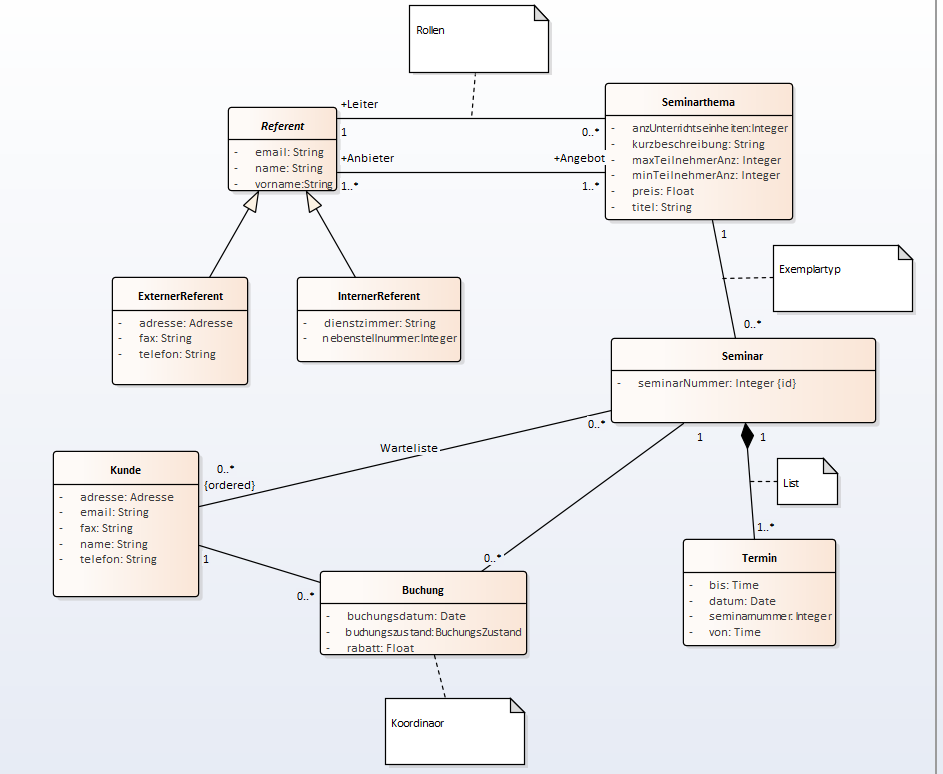
\includegraphics[scale=0.6]{Bilder/diagram02.PNG}
	\caption{OOM Modell}
	\label{er:1}
\end{figure}

Da Vererbung so nicht in einem ER-Modell möglich ist, haben wir eine Anpassung vorgenommen. Ein Interner/Externer Referent hat jeweils noch einen Verweis auf den Eintrag von Referent.
Außerdem haben wir statt einer Klasse Buchung eine Beziehung buchen mit den Attributen aus der Klasse.

\subsection{c)}

Ein \texttt{Referent} kann 0 Seminarthemen leiten, da er auch nur Seminare anbieten kann oder beliebig viele da hier keine Beschränkung vorgegeben war. 
Laut Aufgabe kann ein Seminar von genau einem Referent geleitet werden aber mehrere Anbieter haben. Ein Referent kann gleichzeitig Anbieter und Leiter sein.

Ein Seminarthema kann 0 Seminare haben, um sicherzustellen, dass zur Anmeldung nicht schon ein Seminar eingetragen werden muss. Es kann aber im Laufe mehrere Seminare haben.
In einem Seminar kann nur genau ein Seminarthema behandelt werden.

Ein Seminar kann an mehreren Terminen statt finden. Muss aber an mindestens eins. Ein Termin kann nur zu genau einem Seminar gehören.

Kunden können angelegt werden ohne an einem Seminar teilzunehmen oder auf einer Warteliste zu stehen. Deshalb die 0 Kardinalitäten. Im Laufe können sie aber an beliebig vielen Seminaren teilnehmen oder auf Wartelisten stehen. In die andere Richtung gilt genau das gleiche.


\end{document}



